\chapter{Grundlagen}
\label{sec:state}

% Hier werden zwei wesentliche Aufgaben erledigt:

% 1. Der Leser muß alles beigebracht bekommen, was er zum Verständnis
% der späteren Kapitel braucht. Insbesondere sind in unserem Fach die
% Systemvoraussetzungen zu klären, die man später benutzt. Zulässig ist
% auch, daß man hier auf Tutorials oder Ähnliches verweist, die hier auf
% dem Netz zugänglich sind.
% 2. Es muß klar werden, was anderswo zu diesem Problem gearbeitet
% wird. Insbesondere sollen natürlich die Lücken der anderen klar
% werden. Warum ist die eigene Arbeit, der eigene Ansatz wichtig, um
% hier den Stand der Technik weiterzubringen? Dieses Kapitel wird von
% vielen Lesern übergangen (nicht aber vom Gutachter ;-), auch später
% bei Veröffentlichungen ist "Related Work" eine wichtige Sache.

% Viele Leser stellen dann später fest, daß sie einige der Grundlagen
% doch brauchen und blättern zurück. Deshalb ist es gut,
% Rückwärtsverweise in späteren Kapiteln zu haben, und zwar so, daß man
% die Abschnitte, auf die verwiesen wird, auch für sich lesen
% kann. Diese Kapitel kann relativ lang werden, je größer der Kontext
% der Arbeit, desto länger. Es lohnt sich auch! Den Text kann man unter
% Umständen wiederverwenden, indem man ihn als "Tutorial" zu einem
% Gebiet auch dem Netz zugänglich macht.

% Dadurch gewinnt man manchmal wertvolle Hinweise von Kollegen. Dieses
% Kapitel wird in der Regel zuerst geschrieben und ist das Einfachste
Um einen Überblick in die Grundlagen dieser Bachelorarbeit zu geben, erfolgt in diesem Kapitel zunächst die Erläuterung zentraler Begriffe der Netzwerktheorie. Das ist eine wichtige Voraussetzung, um die Funktionsweise vom Sicherheitsstandard \gls{MACsec} verstehen zu können. Danach werden grundlegende im Standard benutzte Sicherheitsbegriffe beschrieben, um anschließend auf den Standard als solches, dessen Funktion und Sicherheitsziele einzugehen. Falls es nicht anders erwähnt wird, werden die Kenntnisse für den Abschnitt 2.1 aus \cite{TN_libero_mab23259530} entnommen.
\section{Netzwerktheorie}
% (oder das Schwerste weil erste).
%In diesem Kapitel werden als erstes zentrale Begriffe der Netzwerktheorie erklärt, die essentiell sind, um die Funktionsweise vom Sicherheitsstandard MACsec zu verstehen. Danach werden grundlegende Sicherheitsbegriffe und Verfahren darstellen, die im Standard benutzt werden. Anschließend erfolgt die Beschreibung des MACsec Standards,( wie es funktioniert, was geschützt wird und welche Sicherheitsziele verfolgt werden.)
%zentrale Begriffe der Netzwerktheorie und der Kryptographie, die zum Verständnis der Bachelorarbeit essentiell sind, eingeführt und erläutert.
%Um das Verständnis 


\textbf{OSI Referenzmodell} \\
\\
Das OSI Referenzmodell wurde von der \gls{ISO} entwickelt. Es war der erste Versuch  Kommunikationsprotokolle zu standardisieren, um zwischen verschiedenen technischen Systemen zu kommunizieren. Das \gls{OSI-Modell} besteht aus sieben Schichten, wobei jede einzelne Schicht eine genau definierte Funktion erfüllt. Wenn eine Nachricht von einem zum anderen Computer geschickt wird, durchläuft die Nachricht zuerst alle 7 Schichten auf dem Computer des Senders und ein zweites Mal alle 7 Schichten auf dem Computer des Empfängers. Für den Gegenstand der Bachelorarbeit ist die Sicherungsschicht von besonderer Bedeutung, da \gls{MACsec} selbst auf der 2. Schicht des \gls{OSI-Modell}s arbeitet und Kenntnisse aus dieser Schicht relevant zum Verständnis dieser Arbeit sind.\\
\\
\textbf{Sicherungsschicht}\\ 
\\
Die Sicherungsschicht ist die zweite Ebene des \gls{OSI-Modell}s. Ihre Aufgabe ist es den Bitstrom aus der Bitübertragungsschicht (Schicht 1) in Blöcke, die Rahmen genannt werden, aufzuteilen und an die Vermittlungsschicht (Schicht 3) weiterzuleiten. So muss durch die Sicherungsschicht eine zuverlässige Übertragung der Daten gewährleistet werden. Hierfür werden zusätzliche Redundanzen zum Rahmen hinzugefügt, um gesendete Informationen auf Fehler zu prüfen und Maßnahmen der Fehlerkorrektur durchführen zu können. Deshalb muss in der Vermittlungsschicht nicht mehr auf grobe Fehler in dem Datenpaket geprüft werden. Ein weiteres wichtiges Kriterium ist die Regulierung des Datenflusses durch den Empfänger. Dies dient dazu, dass es nicht zu einer Überlastung des Empfängers kommt, falls der Sender schneller Daten sendet als der Empfänger annehmen kann. Die Sicherungsschicht wird in zwei Teilschichten untergliedert, die \gls{MAC} und die \gls{LLC}. \\
\\\\
\textbf{Medium Access Control}\\\\
In der Medium Access Control Teilschicht werden die vorhandenen Kommunikationskanäle zwischen den Mitgliedern innerhalb eines Netzwerks organisiert. Hierbei wird während der Übertragung überprüft, ob es zu einer Kollision auf dem Kanal zwischen den Kommunikationspartnern gekommen ist. Im Falle einer Kollision werden je nach Protokoll unterschiedliche Maßnahmen ergriffen, um die Kollisionsgefahr auf dem Kanal zu verringern. Allerdings müssen bei einer Kollision die Nachrichten generell erneut gesendet werden. In der Literatur findet man auch kollisionsfreie Übertragungsprotokolle, diese finden in der Praxis jedoch kaum Anwendung. 
%In der Medium Access Controll Teilschicht werden Verfahren zur Kollisionsbereinigung 
%broadcast kanal wird mehreren benutzern bereitgestellt, Von %einer Kollision ist die Rede, wenn beide Kommunikationsstationen eine Nachricht zum gleichen Zeitpunkt senden. einer Nachricht auf dem Kanal gemeint. führt zu kollisionen.\\
\\
\\
\textbf{Ethernet}
\\
\\
Ethernet wurde unter dem Begriff \gls{IEEE} Norm 802.3 standardisiert. Daher können \gls{IEEE} Norm 802.3 und Ethernet als Synonym verwendet werden. In dieser Bachelorarbeit wird stets der Begriff Ethernet verwendet, da dies die gängigste Verbreitung des Ausdrucks ist. Ethernet beschreibt im Allgemeinen die physische Verbindung von 2 Systemen mittels eines Kabels, wodurch die Kommunikation der beiden Systeme erfolgt.\\
\\
\begin{figure}
	\centering
	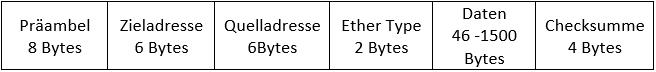
\includegraphics[width=0.9\textwidth]{images/Ethernet_Rahmen.PNG}
	\caption[Felder eines Ethernet Rahmen]{In der Abbildung werden die 6 Bestandteile eines Ethernet Rahmen gezeigt. Dazu wird die Größe eines Feldes in Bytes angezeigt. }
	\label{img:Rahmen}
\end{figure}\textbf{Ethernet auf der MAC-Teilschicht}\\
\\\label{sec: Ethernet auf der MAC-Teilschicht}
Die Daten, die über die \gls{MAC}-Teilschicht des \gls{OSI-Modell}s laufen, werden in der Fachliteratur als Rahmen bezeichnet. Deshalb wird im Verlauf der Arbeit stets der Begriff Rahmen für diese Daten übernommen. Ein Rahmen beim Ethernet in der \gls{MAC}-Teilschicht weist folgende Struktur auf. Als erstes beginnt ein Rahmen mit einer Präambel, die eine Länge von 8 Bytes aufweist, wobei jedes Byte das Bitmuster 10101010 besitzt, ausgenommen sind die letzten beiden Bits. Diese werden auf 11 gesetzt. Dies hat den Zweck, Empfänger und Sender zu synchronisieren. Als nächstes folgen zwei 6 Bytes lange Stücke. Der erste Teil beinhaltet die \gls{MAC}-Addresse des Empfängers und der zweite die des Senders. Eine Besonderheit der \gls{MAC}-Adresse ist dadurch gekennzeichnet, dass die Vergabe nur von der \gls{IEEE} erfolgt und jede \gls{MAC}-Adresse global einzigartig ist. Anschließend wird die Länge des Rahmens in einem 2 Byte großem Feld angegeben. In neueren Ethernet Versionen wird das 2 Byte große Feld zum Typ Feld, sodass Protokolle mittels des Typ Feldes unterschieden werden können. Danach folgt nun das Daten Feld, in denen sich die zu sendenden Daten befinden. Das Daten Feld ist maximal 1500 Bytes groß. Also kann ein Rahmen in der \gls{MAC}-Teilschicht eine maximale Größe von 1518 Bytes haben, wenn man die Größe des Headers und Trailers hinzurechnet. Außerdem gibt es auch eine Mindestgröße des Daten Feldes von 46 Bytes. Sollte eine Nachricht trotzdem kleiner sein, so wird die Nachricht mit Nullen auf 46 Bytes aufgefüllt. Daraus folgt, dass ein kompletter Rahmen mindestens eine Größe von 64 Bytes hat. Dies ist die minimale Größe, die benötigt wird, um die Verfahren zur Kollisionserkennung gewährleisten zu können. Ansonsten ist die ganze Nachricht bereits gesendet, bevor der Empfänger realisieren kann, dass eine Kollision vorlag. Zuletzt kommt ein 4 Byte großes Feld, in dem sich die Checksumme befindet. Durch die Checksumme kann überprüft werden, ob die Nachricht korrekt übertragen wurde. Falls dies nicht der Fall sein sollte, kann der Empfänger ein Signal senden, damit der Sender den Rahmen erneut überträgt. Nach einer übermittelten Nachricht wird eine 9,6 \textmu s lange Sendepause eingelegt.
Die Struktur eines Ethernet Rahmens mit seinen einzelnen Feldern ist in der Abbildung \ref{img:Rahmen} zu sehen. \\
\\
\textbf{ICMP}\\
\\
Das \gls{ICMP} ist ein Steuerprotokoll, welches auf der Vermittlungsschicht arbeitet. Sollte im Verlauf einer Paketübertragung ein Router ausfallen oder ein anderes Problem auftreten, so wird dem Sender durch das \gls{ICMP} ein Paket übermittelt, in dem der Sender über das Ereignis informiert wird. 
%An dieser Stelle sollte hervorgehoben werden, dass nur einige Fehlermeldungen erkannt werden 
Eine Liste der unterstützten Nachrichten findet man unter \cite{ICMP}.\\
\\
\textbf{TCP}
\\
\\
Das \gls{TCP} ist ein Internetübertragungsprotokoll, das eine zuverlässige Übertragung garantiert. Außerdem wird bei \gls{TCP} auf die Reihenfolge der Pakete wert gelegt. Es wird in der der Transportschicht des \gls{OSI-Modell}s, der 4. Schicht, eingesetzt. Auch wenn die vorhandenen Netzwerke unzuverlässig sind, kann sich das \gls{TCP} robust auf alle Arten von Fehlern einstellen. Beim \gls{TCP}-Protokoll werden übertragende Daten als Segmente bezeichnet. Ein \gls{TCP}-Segment fängt mit einem 20-Byte langem Header an, gefolgt von einem optionalen Teil und anschließend von einem Datenbytes-Feld, das auch, anders als bei Ethernet, keine Daten enthalten kann.
\section{Sicherheit}\\
\\
In diesem Abschnitt werden einige Grundlagen der Sicherheit in Rechnernetzen erläutert, die für das Verständnis der Funktionsweise des Sicherheitsstandards MACsec von Bedeutung sind. Die Informationen für diesen Abschnitt sind aus \cite{pfitzmann2000sicherheit} entnommen.
\\
\\
\textbf{Sicherheitsziele}\\
\\
Es wird im Allgemeinen in 3 Sicherheitsziele unterteilt:
\begin{itemize}
\item Vertraulichkeit: Es ist nicht möglich, dass eine unautorisierte Partei einen Informationsgewinn über den Inhalt der gesendeten Daten erhält.
\item Integrität: Es ist nicht möglich, dass eine unautorisierte Partei den Inhalt von Daten modifizieren kann, ohne das dies bemerkt wird.
\item Verfügbarkeit: Es ist nicht möglich, dass eine unautorisierte Partei die Funktionalität eines Dienstes beeinträchtigen kann.
\end{itemize} \\
In dieser Arbeit ist noch ein 4. Sicherheitsziel von Bedeutung:
\begin{itemize}
\item Authentizität: Eine gesendete Nachricht kann einem Sender zugeordnet werden.\\
\end{itemize}
\\
\textbf{Symmetrisches Konzelationssystem}\\
\\
Bei einem symmetrischen Konzelationssystem wird ein zufälliger Schlüssel generiert, der zwischen Sender und Empfänger ausgetauscht wird. Dieser Schlüssel wird sowohl bei der Verschlüsselung als auch Entschlüsselung von Nachrichten angewendet. Mit einem symmetrischen Konzelationssystem kann das Schutzziel der Vertraulichkeit erfüllt werden. \\
\\
\textbf{Symmetrisches Authentikationssystem}\\
\\
%Authentikations oder Authentifikationssytem?
Bei einem symmetrischen Authentikationssystem wird ebenfalls ein zufälliger Schlüssel generiert, der zwischen Sender und Empfänger ausgetauscht wird. Anders als bei einem Konzelationssystem werden die ausgetauschten Nachrichten nicht verschlüsselt und entschlüsselt, sondern es wird ein Prüfteil an die zu sendende Nachricht angefügt. Der Empfänger einer Nachricht kann mit dem richtigen Schlüssel den Prüfteil selbständig berechnen und vergleichen. Sollte sich der berechnete Prüfteil von der erhaltenen Nachricht unterscheiden, dann wurde die Nachricht verändert. Mit einem Authentikationssystem kann das Schutzziel der Integrität erfüllt werden. In der restlichen Arbeit wird der gängigere englische Begriff des Message Authentikation Codes \gls{MAC} anstelle des Authentikationssystems verwendet.\\
\\
\textbf{Replay-Angriff}\\
\\ 
Bei einem Replay-Angriff werden bereits gesendete Nachrichten von einem Angreifer gesammelt und erneut in den Nachrichtenfluss gestreut, meistens mit der Intention das Sicherheitsziel der Authentizität zu schwächen. \\  
\\
\textbf{bounded receive delay}\\
\\
Unter bounded receive delay versteht man, dass ein Man-in-the-Middle Angreifer keine Pakete in einem Netzwerk verzögern oder abfangen kann, ohne das dies von den Beteiligten in einem Netzwerk erkannt wird.
\\
\\
\\
\\
\textbf{Denial of Service}\\
\\
\gls{DoS} ist ein Angriff mit der Absicht, das Sicherheitsziel der Verfügbarkeit zu schwächen. Dazu werden an einen Server eine Vielzahl von Anfragen geschickt, bis der Server überlastet ist und diese nicht mehr beantworten kann. Der Server kann zu diesem Zeitpunkt keine sinnvollen Anfragen von Nutzern mehr beantworten, die auf den Service des Servers zugreifen wollen. Somit ist der Service für die Nutzer nicht mehr verfügbar.
\section{Authenticated Encryption with Associated Data}
\label{sec:Authenticated Encryption with Associated Data}
\\
\\
Authenticated Encryption with Associated Data (\gls{AEAD}) ist ein  Betriebsmodus, in dem ein Konzelationssystem und ein Authentikationssystem in einem Verschlüsselungsprotokoll vereint werden. Dabei ist es nicht unüblich, dass zwei unterschiedliche Algorithmen, eine Stromchiffre und ein Message Authentikation Code zu einen Schema verbunden werden.  
Um mittels \gls{AEAD} verschlüsseln zu können, braucht man folgende Inputs:
\begin{itemize}
\item den \gls{K}
\item den \gls{IV}
\item die \gls{AD}
\item den \gls{M}
\end{itemize} \\
Die \gls{AD} ist ein zusätzlicher Input, der zu dem Verschlüsselungsprotokoll hinzugefügt wird, aber intern nicht verschlüsselt wird. Vielmehr wird die \gls{AD} in den Zustand des Algorithmus geladen, um das Schutzziel der Authentizität zu erreichen. Im \gls{MACsec} Protokoll werden Teile des \gls{MACsec} Headers wie Sende- und Empfängeradresse als Associated Data benutzt. Das wird später in \ref{sec:Media Access Control Security - MACsec} erläutert. Die Länge des symmetrischen Schlüssels und die Länge des Initialisierungsvektors muss nicht gleich sein. So ist zum Beispiel die Länge des Schlüssels bei \gls{AES-GCM} 128 Bit lang, wobei der selbe Algorithmus nur einen 96 Bit langen Initialisierungsvektor verwendet. Allerdings verlieren die meisten \gls{AEAD} Algorithmen ihre Sicherheit, wenn der gleiche Schlüssel mit dem gleichen Initialisierungsvektor benutzt wird. Daher muss \gls{AES-GCM} mit einem kürzeren \gls{IV} öfter den Schlüssel wechseln als andere Algorithmen, die einen längeren Initialisierungsvektor benutzen. \\
Als Output bekommt man einmal das \gls{C} und den MAC (T), der unter anderem auch als Tag bezeichnet wird. Der MAC wird an die verschlüsselte Nachricht konkateniert, sodass am Ende des Verschlüsselungsprotokolls die Nachricht um die Länge des MACs vergrößert wird. Wie bereits erwähnt, kann über den MAC das Schutzziel der Integrität erreicht werden. Dadurch, dass am Anfang die \gls{AD} in den Algorithmus geladen wird, kann auch über den MAC die Authentizität des Senders bestätigt werden.\\
\\
Zum Entschlüsseln benötigt man 4 Inputs:
\begin{itemize}
\item Den Schlüssel (\gls{K})
\item den Initialisierungsvektor (\gls{IV})
\item die associated Data (\gls{AD})
\item das Chiffrat (\gls{C})
\end{itemize} Während der Entschlüsselung wird aus dem erhaltenden Chiffrat ein MAC errechnet. In diesem Vorgang wird der errechnete MAC mit dem gesendeten verglichen und bei erfolgreicher Validierung wird die Nachricht ausgegeben. Sollte sich dabei herausstellen, dass der MAC nicht korrekt ist, wird bei diversen \gls{AEAD} Algorithmen empfohlen, den produzierten MAC nicht auszugeben, da sonst die Algorithmen anfällig gegenüber known-plaintext oder chosen-ciphertext Angriffen sind \cite{rfc5116}.

%sagen warum aead vorteile gegenüber anderen betriebsmodi hat!
%Konzelationssysteme und Authentikationssysteme
\subsection{Generische AEAD Algorithmen}
\\
\\
Ein beliebter Grundgedanke, um einen \gls{AEAD} Algorithmus zu erstellen, ist die Kombination aus einer effizienten Stromchiffre mit einem schnellen Message Authentikation Code. Diesen Ansatz bezeichnet man als generische \gls{AEAD} Algorithmen. Um die geforderten Sicherheitsziele der Vertraulichkeit, Authentizität und Integrität zu garantieren, müssen 2 Bedingungen erfüllt werden:
\begin{enumerate}
\item Der Verschlüsselungsalgorithmus muss gegen einen chosen-plaintext Angriff sicher sein.
\item Der Message Authentication Code muss fälschungssicher bei chosen-message Angriffen sein.
\end{enumerate} 
Es gibt 3 Methoden, um einen generischen \gls{AEAD} Algorithmus zu bilden. \\
Die 1. Variante nennt sich Encrypt-and-MAC. Bei Encrypt-and-MAC wird der Klartext verschlüsselt und es wird ein Tag vom Klartext gebildet. Anschließend wird der Tag an den Ciphertext konkateniert. Bei der Verschlüsselung wird als erstes der Ciphertext entschlüsselt. Anschließend wird aus dem Klartext ein Tag berechnet und mit dem erhaltenen Tag verglichen. \\Eine weiterere Möglichkeit nennt sich MAC-then-encrypt. Wenn MAC-then-encrypt verwendet wird, dann wird als erstes ein MAC an den Klartext konkateniert. Daraufhin wird der komplette Klartext mit dem MAC verschlüsselt. Um den MAC zu verifizieren, muss als erstes die komplette Nachricht entschlüsselt werden. Dann wird aus dem Klartext ein MAC berechnet und verglichen.\\
Die letzte Variante wird als Encrypt-then-MAC bezeichnet. Es ist das sicherste Verfahren, bei der als erstes die Nachricht verschlüsselt und danach aus dem Ciphertext der MAC gebildet wird. Bei der Authentifizierung der Nachricht erfolgt die Berechnung des MAC aus dem Ciphertext. Im Anschluss findet der Vergleich mit den beiden MACs statt und bei erfolgreicher Validierung folgt die Entschlüsselung des Ciphertextes \cite{10.1007/3-540-44448-3_41}. 
\\
\\

%\textbf{Differentielle Kryptoanalyse}\\
%\\ Die differentielle Kryptoanalyse ist ein statistischer Angriff auf rundenbasierten Blockchiffren, die auf dem verbreiteten Substitutions-/Permutations-Netz (SPN) basieren. Das Ziel dieses Angriffs ist es den gesamten Schlüssel oder Teile davon zu berechnen, in dem man die Differenzen zwischen Klartextblöcken und den erzeugten Ciphertextblöcken vergleicht. %%geht noch ein bisschen besser oder genauer
\section{Media Access Control Security - MACsec}
\label{sec:Media Access Control Security - MACsec}
\\
\\
Media Access Control Security \gls{MACsec} ist ein Sicherheitsprotokoll, welches von dem Institute of Electrical and Electronics Engineers \gls{IEEE} veröffentlicht worden ist. Es ist auch unter dem Begriff IEEE 802.1AE bekannt. Das Sicherheitsprotokoll \gls{MACsec} bietet Schutz auf der 2. Ebene des \gls{OSI-Modell}s und ist in der Lage, Integrität, Vertraulichkeit und Authentizität zu gewährleisten, weil es das Verschlüsselungsschema \gls{AEAD} verwendet.
Soweit es nicht anders erwähnt wird, werden die Informationen für dieses Kapitel aus \cite{1678345} entnommen.\\
\\
\begin{figure}
\centering
	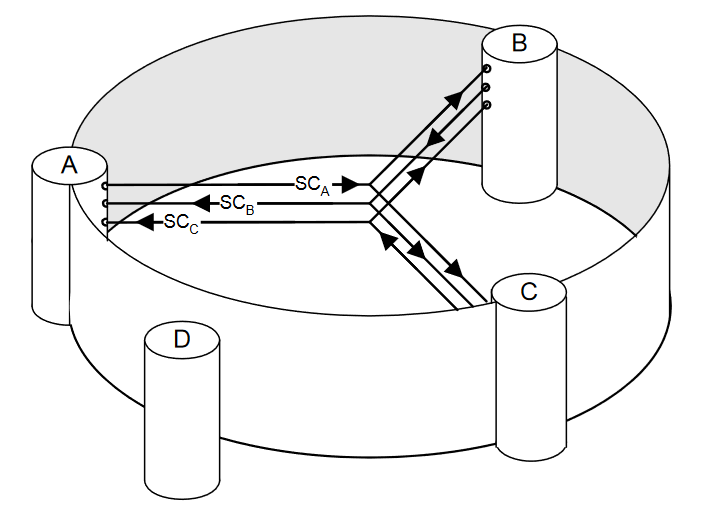
\includegraphics[width=0.85\textwidth]{images/MACsec_CA.PNG}
	\caption[Modell der MACsec Connectivity Association]{In dieser Abbildung werden 3 Stationen gezeigt, die sich in eine Connectivity Association befinden und mittels Secure Channel kommunizieren können.  }
	\label{img:MACsec_CA}
\end{figure}\gls{MACsec} kann eine sichere Kommunikation in einem LAN-Netzwerk bereitstellen. Um das \gls{MACsec} Protokoll verwenden zu können, muss jeder Nutzer eine \gls{SecY} und eine \gls{KaY} benutzen. Eine \gls{SecY} ist eine Instanz des \gls{MACsec} Protokolls, die alle Operationen ausführt, die im MACsec Standard beschrieben werden. Allerdings kann die \gls{SecY} nicht zwischen Nutzern, die das \gls{MACsec} Protokoll benutzen und normalen Nutzern unterscheiden. Um Nutzer authentifizieren zu können, wird die \gls{KaY} benötigt. Die \gls{KaY} ist für den Schlüsselaustausch, die Bereitstellung der Schlüssel, für die Autorisierung und Authentifizierung von anderen Nutzern mit einer \gls{SecY} verantwortlich. Hierfür ist ein eigener Standard, das \gls{MKA} entstanden\cite{5409813}.\\
Ein Nutzer mit einer \gls{SecY} kann in genau eine \gls{CA} eintreten. \gls{CA} bilden sichere Umgebungen, in denen die Mitglieder miteinander kommunizieren können. Nur die \gls{KaY} kann Nutzer innerhalb einer \gls{CA} erkennen. Eine \gls{MACsec} \gls{SecY} muss sich indes gar nicht bewusst sein, dass sie sich in einer \gls{CA} befindet. Wenn sich zwei \gls{SecY} innerhalb einer \gls{CA} befinden, so können sie über einen \glspl{SC} miteinander kommunizieren. Ein \gls{SC} wird auf 4 \glspl{SA} aufgeteilt. Jede Secure Association besitzt ihren eigenen \gls{SAK}, ein Schlüssel, der durch die \gls{KaY} bereitgestellt wird. Jede \gls{SA} wird durch einen \gls{SCI} identifiziert. Der Empfänger einer Nachricht kann durch den \gls{SCI} eine \gls{SA} erkennen, was wichtig ist, um den richtigen Schlüssel für die Entschlüsselung zu wählen.
 \ref{img:MACsec_CA} zeigt die \gls{SC} zwischen mehreren \gls{SecY} innerhalb eines \gls{CA}.
\subsection{MACsec auf Layer 2} \\
\label{sec:MACsec Layer 2}
\\
\begin{figure}
	\centering
	\includegraphics{images/MACsec_Frame.PNG}
	\caption[MACsec Rahmen]{In der Abbildung werden die Änderungen veranschaulicht, die der MACsec Standard an einem Rahmen vornimmt. Die grün und rot markierten Felder werden vom ICV geschützt. Das rote Feld beschreibt zudem das Nutzdaten Feld, welches verschlüsselt werden kann.}
	\label{img:MACsec_Frame}
\end{figure}Wie bereits erwähnt, arbeitet \gls{MACsec} auf der zweiten Ebene des \gls{OSI-Modell}s. Wird ein Paket über \gls{MACsec} verschickt, dann verändert \gls{MACsec} den Rahmen. Es wird ein zusätzliches Feld der SecTag angefügt und der Ethertype des Rahmens wird auf 0x88e5 gesetzt, den Ethertype von \gls{MACsec}. Zusätzlich wird ein \gls{ICV} nach dem Daten Feld konkateniert. Der \gls{ICV} wird durch den Message Authentication Code, der in \gls{MACsec} genutzt wird, gebildet. Als Input wird der SecTag, der Ethertype und das Daten Feld genommen,  sodass der \gls{ICV} alle wichtigen Bestandteile des Rahmens schützt. Es gibt in \gls{MACsec} mehrere Möglichkeiten, um einen Rahmen zu schützen. Man kann die Vertraulichkeit und Integrität oder nur Integrität schützen. Bei Vertraulichkeit und Integrität wird als erstes das Daten Feld verschlüsselt und dann der \gls{ICV} über den kompletten Rahmen gebildet. Wenn man nur Integrität auswählt, dann wird nur ein \gls{ICV} gebildet.
Die Änderungen am Rahmen ermöglichen \gls{MACsec} Angriffsmöglichkeiten wie Replay Angriffe und Denial of Service zu unterbinden. Außerdem lehnt MACsec Rahmen ab, die eine zu lange Übertragungszeit haben. Damit wird ein möglicher bounded receive delay unterbunden.
In der Abbildung \ref{img:MACsec_Frame} wird ein MACsec Rahmen dargestellt. Die grün und rot markierten Felder werden vom ICV geschützt. Das rote Feld zeigt die verschlüsselten Daten.
\\
\\
\textbf{MACsec SecTag}
\\
\\
\begin{figure}
	
	\centering 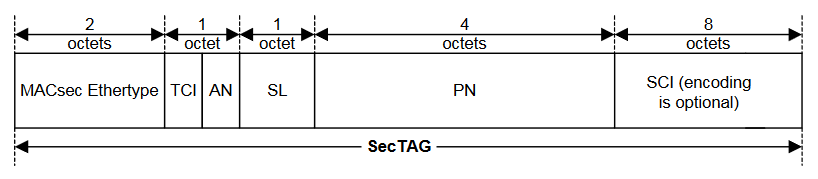
\includegraphics[width=0.9\textwidth]{images/SecTag_Format.PNG}
	\caption[SecTag Header vom MACsec Standard]{Die Abbildung zeigt den SecTag Header des MACsec Standards. Darin sind die einzelnen Felder und deren Größe in Bytes zu erkennen.}
	\label{img:SecTag}
\end{figure}Der SecTag ist ein zusätzlicher Header, der zwischen dem Ethertype Feld und dem Daten Feld eines \gls{MACsec} Rahmens eingefügt wird. Je nach Auswahl besitzt der SecTag eine Größe von 8 oder 16 Bytes und besteht aus folgenden Feldern: 
\begin{itemize}
\item dem Ethertype mit einer Größe von 2 Bytes.
\item der Tag Control Information mit einer Größe von 6 Bits.
\item der Association Number mit einer Größe von 2 Bits.
\item dem Short Field mit einer Größe von 1 Byte.
\item der Paket Nummer mit einer Größe von 4 Bytes.
\item dem SCI ein Optionales Feld mit einer Größe von 8 Bytes.
\end{itemize} \\
Ob ein Rahmen durch ein Protokoll genutzt oder verändert worden ist, kann man an dem Ethertype Feld erkennen. Bei MACsec hat das Ethertype Feld den statischen Wert 0x88E5. Darauf folgt das \gls{TCI}, das im nächsten Absatz näher erläutert wird. 
Die \gls{AN} wird mit dem Secure Channel Identifier konkateniert, um eine Secure Association zu erkennen. 
Danach kommt das Feld Short Field. Dieses Feld ist in der Regel auf 0 gesetzt. Sollte allerdings ein Paket kürzer, als die von \gls{MACsec} vorausgesetzten 48 Bytes sein, wird in diesem Feld die Länge des Pakets als Integer angegeben. 
%wird dann gepadded?
Die Paketnummer ist Teil des Initialisierungsvektors. Jedes Paket, das gesendet wird, bekommt seine eigene Paketnummer, die inkrementiert wird und somit immer unterschiedlich ist. %verweis auf den aead abschnitt
Zum Schluss kommt das optionale Feld mit dem Secure Channel Identifier. Der \gls{SCI} wird nur aktiviert, wenn das \gls{SC} Bit im \gls{TCI} gesetzt ist. Mit dem \gls{SCI} und der \gls{AN} kann man zusammen die \gls{SA} bestimmen. Das ist besonders wichtig, da jede \gls{SA} ihren eigenen \gls{SAK} besitzt. Somit muss erkannt werden, in welcher \gls{SA} die Nachricht übermittelt worden ist, um den richtigen Schlüssel zur Entschlüsselung zu benutzen. Des Weiteren wird der \gls{SCI} genutzt, um die \gls{SecY} zu identifizieren, die einen Rahmen zur Station gesendet hat. Wird kein SCI benutzt, so übermittelt das \gls{MKA} einen Wert und eine Verbindung mittels \gls{PPP} wird erstellt. In der Abbildung \ref{img:SecTag} werden die einzelnen Bestandteile eines MACsec SecTag dargstellt. Zusätzlich wird die Größe jedes Feldes in Bytes angezeigt.\\
\\
\textbf{MACsec Tag Control Information}\\
\\
\begin{figure}
	
	\centering 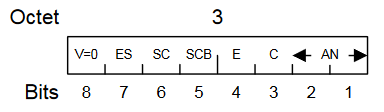
\includegraphics[width=0.65\textwidth]{images/TAG_Feld.PNG}
	\caption[Tag Control Information Feld]{In der Abbildung werden die einzelnen Bits des Tag Control Information Feldes aufgezeigt.}
	\label{img:TAG_Feld}
\end{figure}Das Tag Control Information Feld ist Bestandteil des \gls{MACsec} SecTag Headers. Das \gls{TCI} ist nur 6 Bits lang, allerdings hat jedes Bit eine feste Funktion.
Das erste Bit steht für die Versionsnummer. Im Standard wird angemerkt, dass in der Zukunft mehr als ein Bit benötigt werden, um die Versionsnummer anzuzeigen.
Das zweite Bit steht für das \gls{ES}. Das ES Bit wird nur gesetzt, wenn die ersten 6 Bytes des \gls{TCI} identisch zu den ersten 6 Bytes der MAC Adresse sind. Ist das ES Bit gesetzt, so wird vom Standard \cite{1678345} empfohlen, das SCI nicht direkt im SecTag zu kodieren und das SC Bit nicht zu setzen.
Wenn ein SCI benutzt wird, ist das SC Bit aktiv.
Nur wenn ein MACsec Rahmen mit einem Secure Channel assoziiert wird und EPON Single Copy Broadcast capability unterstützt, dann wird das SCB Bit gesetzt.
Das E Bit ist gesetzt, wenn das Secure Payload Feld verschlüsselt werden soll.
Das letzte Bit von der \gls{TCI} ist das Changed Text Bit. Ist das E Bit gesetzt und das Changed Text Bit, so wurden erfolgreich die Nutzdaten durch die \gls{SecY} verarbeitet. Ist das E Bit gesetzt, aber das Changed Text Bit noch nicht, dann wurden die Nutzdaten noch nicht durch die SecY verändert.
In der Abbildung \ref{img:TAG_Feld} ist das 6-Bit lange TCI Feld mit seinen einzelnen Komponenten und der \gls{AN} dargestellt.
\\
\\
\textbf{MACsec Secure Data}\\
\\
Das Secure Data Feld beschreibt die Nutzdaten zwischen dem SecTag und dem ICV. Das Feld kann nicht leer sein und muss  eine Länge von mindestens 48 Bytes haben, da dies die kleinste Größe eines Rahmens im Ethernet Standard ist. Ist es kürzer, dann erfolgt die Nutzung von Padding. \\
\\
\textbf{Integrity Check Value}\\
\\
Der Integrity Check Value überprüft, ob eine Nachricht manipuliert worden ist. Im MACsec Standard ist der \gls{ICV} zwischen 8 und 16 Bytes lang, je nachdem welche Cipher Suite ausgewählt worden ist. Wenn der vom Standard empfohlene Algorithmus \gls{AES-GCM} ausgewählt ist, beträgt die Länge 16 Bytes.
\subsection{MACsec Cipher Suite}\\
\\ 
In der Cipher Suite werden alle kryptografischen Algorithmen spezifiziert, die in MACsec angewendet werden können. Zu diesem Zeitpunkt befindet sich nur \gls{AES-GCM} mit einer Schlüssellänge von 128 Bit in der Cipher Suite von \gls{MACsec}. Es ist bereits eine Erweiterung der Cipher Suite geplant, in der AES-GCM mit einer Schlüssellänge von 256 Bit hinzugefügt werden soll\cite{6047536}.
Will man einen weiteren Algorithmus zur Cipher Suite hinzufügen, so müssen folgende Bedingungen erfüllt werden:
\begin{itemize}
\item Durch den Algorithmus müssen die Parameter \gls{SCI}, Paketnummer, Source Address, Destination Address, SecTag und die Nutzdaten geschützt werden. 
\item Der Algorithmus muss sowohl Integrität als auch Vertraulichkeit schützen können. 
\item Ein Verschlüsselungsalgorithmus muss bis zu 2\textsuperscript{32} -1 mal aufrufbar sein, ohne das der \gls{SAK} gewechselt werden muss.
\end{itemize} \\
\textbf{Default Cipher Suite AES-GCM}\\
\\
Die empfohlene Cipher von MACsec ist \gls{AES-GCM} auch bekannt unter \gls{AES} im Galois Counter Mode.  %etwas über die geschichte von gcm(aes) sagen.
2007 wurde AES-GCM von der amerikanischen Bundesbehörde \gls{NIST}, die auch schon den \gls{DES} und AES standardisiert hat, ein Paper veröffentlicht, in dem AES-GCM empfohlen wurde.
Es ist eine generische \gls{AEAD} Cipher, die aus der Stromchiffre AES-CTR mit einer Blocklänge von 128 Bits besteht und aus dem Message Authentikation Code GMAC, der die \gls{ICV} von MACsec mit einer Länge von 128 Bits berechnet. Wie bereits bei \ref{sec:Authenticated Encryption with Associated Data} erwähnt, benötigt ein \gls{AEAD} Schema einen fest definierten Input, der wie folgt aussieht:\\\centerline{(C,T) =\textit{enc}(IV,M,A,K)}\\
Die Schlüssellänge von \gls{AES-GCM} ist 128 Bits lang und als Schlüssel wird der \gls{SAK} einer \gls{SA} benutzt. Die ersten 64 Bits von dem 96 Bits langen \gls{IV} bestehen aus dem SCI. Die restlichen 32 Bits bilden die iterierende Paket Number.
Der Input der \gls{AD} ist die Konkatenation der Destination Mac Adresse, der Source Mac Adresse, des SecTags und zum Schluss der Nutzdaten. Die Argumente werden auch in der genannten Reihenfolge in den Algorithmus geladen.
Unter Anderem bietet MACsec 3 Möglichkeiten an, um eine Nachricht zu schützen:\\
1. Wenn MACsec nur die Integrität einer Nachricht sichern soll, dann ist der Input der Nachricht(M) leer. Die restlichen Parameter werden wie oben beschrieben als Input genommen. Die Secure Data(C) ist in diesem Fall unverändert und es folgt ein 128 Bit langer \gls{ICV}, der die Nachricht schützt.\\
2. Wenn Vertraulichkeit und auch Integrität einer Nachricht geschützt werden sollen, dann muss man einmal unterscheiden, ob man die Nachricht mit einem confidentiality offset oder ohne confidentiality offset verschlüsseln möchte.\\
2.1 Wird mit einem confidentiality offset verschlüsselt, dann wird ein fest auswählbarer Wert z.B. 30 Bytes von der Nachricht (M) nicht verschlüsselt, sondern nur mittels Integrität geschützt. Also die ersten Bytes von der Nachricht direkt nach dem SecTag sind in Klartext verfügbar, werden aber trotzdem durch den \gls{ICV} geschützt. Der Teil der Nachricht, der nicht zum confidentiality offset gehört, wird normal verschlüsselt, ist aber nicht durch den ICV geschützt. Die Secure Data ist der confidentiality offset konkateniert mit den chiffrierten Nutzdaten. \\
2.2 Wird ohne confidentiality offset verschlüsselt, dann wird das gesamte Nutzdaten Feld chiffriert. Die \gls{AD} wird wie oben beschrieben behandelt.
 %diagramm zu ad machen mit option auf confidentiality offset. 
\section{Softwareoptimierung}
Softwareoptimierungen sind angepasste Implementationen, sodass die bestehenden Hardware Unterstützungen von Systemen besser genutzt werden können, um dadurch eine Performance Steigerung zu erreichen. Es gibt Hardware Unterstützungen, die besonders nützlich für Verschlüsselungsalgorithmen sind. Das liegt daran, dass sich die CPU Instruktionen besonders gut dafür eignen, um die verwendeten mathematische Operationen in Verschlüsselungsalgorithmen zu berechnen. Viele Chiffren machen von Software Optimierungen Gebrauch und der AES Verschlüsselungsalgorithmus besitzt sogar einen eigenen Hardware Befehlssatz namens \gls{AES-NI}. In diesem Abschnitt wird daher ein Übersicht über die gängigsten Hardware Unterstützungen geschaffen, die von Verschlüsselungsalgorithmen benutzt werden.
\subsection{AES-NI}
Wie bereits erwähnt, verfügt der Verschlüsselungsalgorithmus \gls{AES} über einen eigenen Befehlssatz AES New Instructions kurz \gls{AES-NI}. Die Befehlssatzerweiterung ist seit 2010 in x86-Prozessoren zu finden. Damit werden 7 zusätzliche Assemblerbefehle unterstützt, die unter anderem Befehle für eine Verschlüsselungsrunde, eine Entschlüsselungsrunde und der Schlüsselgenerierung von AES unterstützt. In \cite{gueron2010intel} wird außerdem gezeigt, dass durch AES-NI die Performance um das 2-3 Fache gesteigert werden kann. Es wird sogar geschildert, dass AES-NI die Sicherheit von AES erhöhen kann, da durch die Instruktionen side-channel Schwächen in der Software von AES verringert werden.
\subsection{SSE}
Eine weitere wichtige Befehlssatzerweiterung ist die \gls{SSE}. SSE bringt 70 Befehlsinstruktionen mit sich und wurde bereits 1999 in x86-Prozessoren unterstützt. Aufgrund der Verwendbarkeit der Instruktionen ist der Befehlssatz in fast jedem x86-Prozessor verfügbar und seitdem sind sogar mehrere Nachfolger von SSE wie z.B SSE2 oder AVX erschienen. In SSE gibt es bis zu 16 128-Bit große Register, die über Vektor Operationen manipuliert werden können. Das hat zur Folge, dass mehrere Befehle an einem Register gleichzeitig durchgeführt werden können. Aus diesem Grund hängt es von der Parallelisierbarkeit des Verschlüsselungsalgorithmus ab, wie sehr die Chiffre vom Befehlssatz profitieren kann\cite{Ankele2016SoftwareBO}.
\subsection{AVX}
Die Advanced Vector Extensions Befehlssatzerweiterung AVX ist wie bereits erwähnt ein Nachfolger von \gls{SSE}. Bei AVX wurden die 16 128-Bit Register auf 16 256-Bit Register mit neuen Instruktionen erweitert. Das Prinzip bleibt das gleiche. Es können mit Vektor Operationen parallel mehrere Befehle an einem Register ausgeführt werden. Durch die 256-Bit großen Register können doppelt so viele Daten simultan verarbeitet werden\cite{mosnavcekoptimizing}.

%%% Local Variables:
%%% TeX-master: "diplom"
%%% End:
